\section{Abstract File System}

图 \ref{fig:architecture} 是这个类的层次结构图。
\begin{figure}
\centering
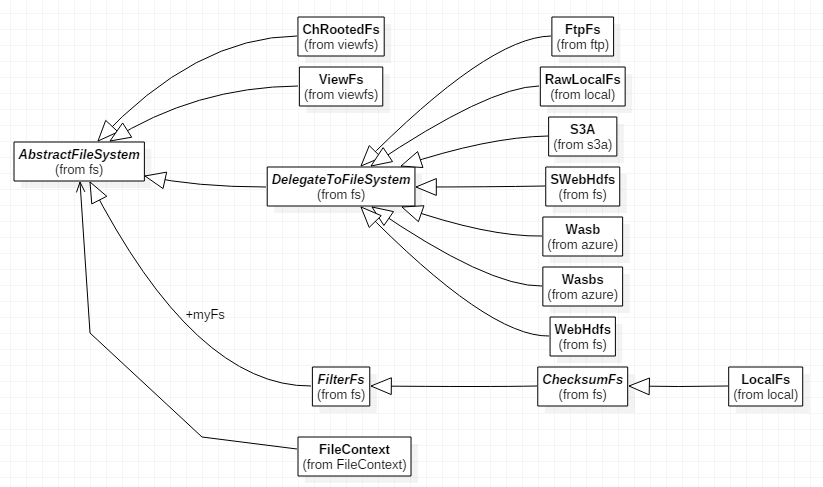
\includegraphics[width=1\linewidth]{UML/abstractfilesystem/architecture.PNG}
\caption{Abstract File System 的层次结构图}
\label{fig:architecture}
\end{figure}

\subsection{AbstractFileSystem}
Abstract File System类是一个抽象类,为Hadoop文件系统的实现者提供了一个接口(类似于Unix的VFS)。应用程序不访问此类,而是使用FileContext 访问所有文件系统中的文件。传递给AbstractFileSystem的路径名可以是与“this”文件系统(即相同的方案和权限)匹配的完全限定URI,或者假定相对于“this”文件系统的根目录的Slash相对名称。

\subsubsection{AbstractFileSystem类图}
图 \ref{fig:abstractFileSystem1}  \ref{fig:abstractFileSystem2} 是这个类的UML类图。

\begin{figure}
\centering
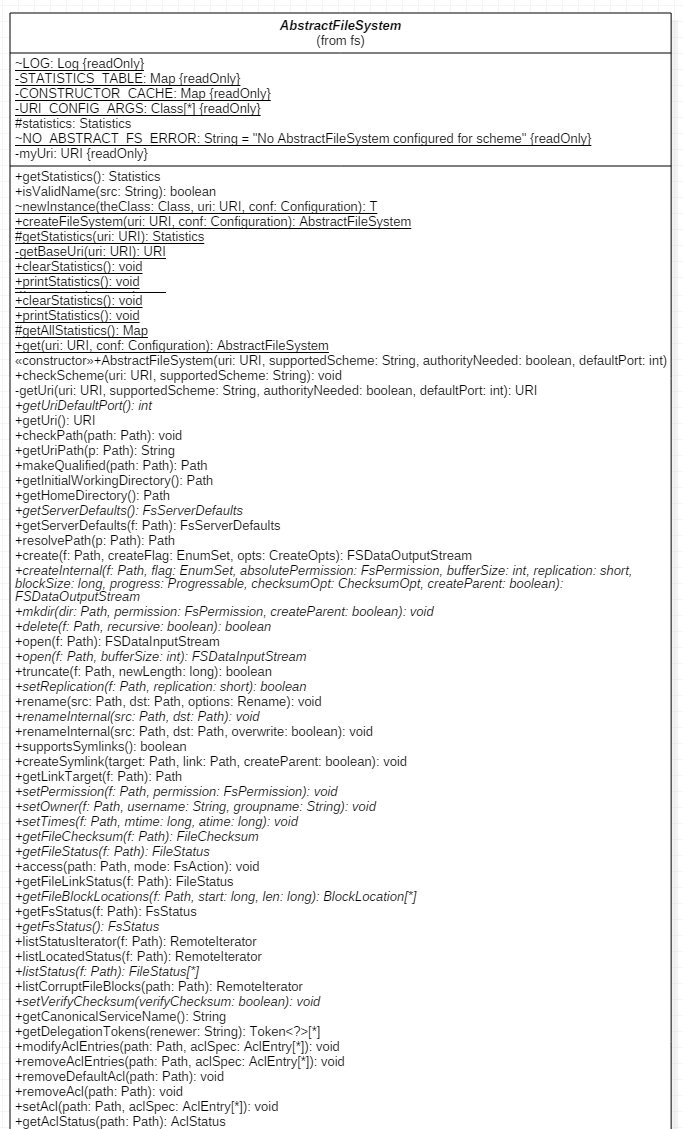
\includegraphics[width=1\linewidth]{UML/abstractfilesystem/abstractFileSystem1.PNG}
\caption{Abstract File System 的UML类图1}
\label{fig:abstractFileSystem1}
\end{figure}

\begin{figure}
\centering
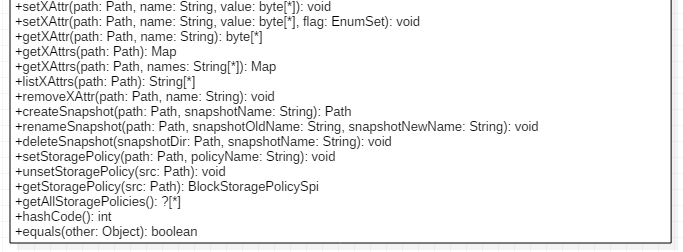
\includegraphics[width=1\linewidth]{UML/abstractfilesystem/abstractFileSystem2.PNG}
\caption{Abstract File System 的UML类图2}
\label{fig:abstractFileSystem2}
\end{figure}
从类图中我们可以看到,该类有对文件系统的基本操作。它与FileSystem有很多同名的方法,这些方法完成相同的功能,比如create,open,delete等等。getstatistics方法对于给定的文件系统获取统计数据。getinitialworkingdirectory方法获取文件系统初始工作目录。还有一些获取扩展属性的方法。

\subsubsection{get方法}
get方法是用于创建文件系统的主要工厂方法,获取uri的scheme和authority。uri的scheme确定一个配置属性名称fs.abastractfilesysytme.scheme.impl,将uri 和conf传递给createfilesystem函数。然后newInstance返回一个AbstractFileSystem的对象。
\begin{java}
  public static AbstractFileSystem get(final URI uri, final Configuration conf)
      throws UnsupportedFileSystemException {
    return createFileSystem(uri, conf);
  }

    /**
   * Create a file system instance for the specified uri using the conf. The
   * conf is used to find the class name that implements the file system. The
   * conf is also passed to the file system for its configuration.
   */
  public static AbstractFileSystem createFileSystem(URI uri, Configuration conf)
      throws UnsupportedFileSystemException {
    final String fsImplConf = String.format("fs.AbstractFileSystem.%s.impl",
        uri.getScheme());

    Class<?> clazz = conf.getClass(fsImplConf, null);
    if (clazz == null) {
      throw new UnsupportedFileSystemException(String.format(
          "%s=null: %s: %s",
          fsImplConf, NO_ABSTRACT_FS_ERROR, uri.getScheme()));
    }
    return (AbstractFileSystem) newInstance(clazz, uri, conf);
  }
\end{java}






\subsection{DelegateToFileSystem}
代理类是对各个具体的文件系统进行封装。抽象文件系统与fs不不同的是,fs的文件系统基本都是fs的直接子类。而在abstractfilesystem中很多文件系统都由delegatetofilesystem 代理。这些被代理的文件系统功能基本相同,实现只有些微的区别。
\subsubsection{DelegateToFileSystem类图}
图 \ref{fig:DelegateToFileSystem} 是这个类的UML类图。
\begin{figure}
\centering
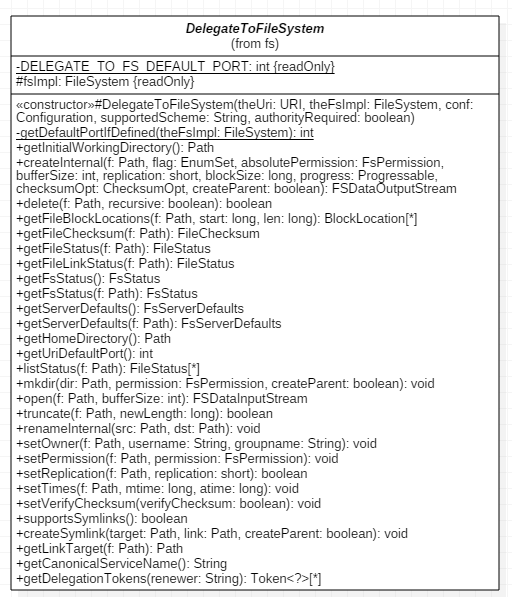
\includegraphics[width=1\linewidth]{UML/abstractfilesystem/DelegateToFileSystem.PNG}
\caption{DelegateToFileSystem的UML类图}
\label{fig:DelegateToFileSystem}
\end{figure}

\subsubsection{fsImpl}
在DelegateToFileSystem类中,有一个FileSystem类型的属性protected final FileSystem fsImpl,DelegateToFileSyste类的初始化要依靠这个属性。
\begin{java}
protected DelegateToFileSystem(URI theUri, FileSystem theFsImpl,
      Configuration conf, String supportedScheme, boolean authorityRequired)
      throws IOException, URISyntaxException {
    super(theUri, supportedScheme, authorityRequired,
        getDefaultPortIfDefined(theFsImpl));
    fsImpl = theFsImpl;
    fsImpl.initialize(theUri, conf);
    fsImpl.statistics = getStatistics();
  }
\end{java}

\subsubsection{S3A}
S3:Amazon S3(Simple Storage Service)是一种数据存储服务。
S3a:自Hadoop2.7以后运用的是s3a,s3a可支持较大的文件,具有更高的性能。替代以前的s3n.
构造函数中的new S3AFileSystem()是通过DelegateToFileSystem 中的FileSystem类型的属性完成的。
\begin{java}
/**
 * S3A implementation of AbstractFileSystem.
 * This impl delegates to the S3AFileSystem
 */
public class S3A extends DelegateToFileSystem{

  public S3A(URI theUri, Configuration conf)
          throws IOException, URISyntaxException {
    super(theUri, new S3AFileSystem(), conf, "s3a", false);
  }

  @Override
  public int getUriDefaultPort() {
    return Constants.S3A_DEFAULT_PORT;
  }
}
\end{java}

\subsubsection{RawLocalFs}
RawLocalFs是不带校验和的原生本地文件系统。
\begin{java}
/**
 * The RawLocalFs implementation of AbstractFileSystem.
 *  This impl delegates to the old FileSystem
 */

public class RawLocalFs extends DelegateToFileSystem {

  RawLocalFs(final Configuration conf) throws IOException, URISyntaxException {
    this(FsConstants.LOCAL_FS_URI, conf);
  }

  /**
   * This constructor has the signature needed by
   * {@link AbstractFileSystem#createFileSystem(URI, Configuration)}.
   */
  RawLocalFs(final URI theUri, final Configuration conf) throws IOException,
      URISyntaxException {
    super(theUri, new RawLocalFileSystem(), conf,
        FsConstants.LOCAL_FS_URI.getScheme(), false);
  }

  //......
}
\end{java}

\subsubsection{WebHdfs}
提供对HDFS的安全读写访问的文件系统,它利用的是http协议。旨在替代HFTP和HSFTP。hftp是在http上提供对hdfs只读访问的文件系统,虽然其名称为hftp但它与ftp无关。
\begin{java}
/**
 * AbstractFileSystem implementation for HDFS over the web.
 */
public class WebHdfs extends DelegateToFileSystem {

  public static final String SCHEME = "webhdfs";

  /**
   * This constructor has the signature needed by
   * {@link AbstractFileSystem#createFileSystem(URI, Configuration)}
   *
   * @param theUri which must be that of webhdfs
   * @param conf   configuration
   * @throws IOException
   */
  WebHdfs(URI theUri, Configuration conf)
      throws IOException, URISyntaxException {
    super(theUri, createWebHdfsFileSystem(conf), conf, SCHEME, false);
  }

  /**
   * Returns a new {@link WebHdfsFileSystem}, with the given configuration.
   */
  private static WebHdfsFileSystem createWebHdfsFileSystem(Configuration conf) {
    WebHdfsFileSystem fs = new WebHdfsFileSystem();
    fs.setConf(conf);
    return fs;
  }
}
\end{java}


\subsection{FilterFs}
一个FilterFs包含一些作为基本文件系统的其它的文件系统,会提供数据转换等附加功能。这个类FilterFs本身就是简单的覆盖所有版本的AbstractFileSystem 的方法,将所有请求传递给包含的文件系统的子类。FilterFs可以进一步覆盖这些方法中的一些,也可以提供其他方法和域。FilterFs类中拥有一个AbstractFileSystem类型的属性myFs。FilterFs 将其作为基本的文件系统。FilterFs 类几乎将所有重写的方法交给了其内部保存的myFs 来处理。但在交给myFs 处理之前,自己可以做一些处理,以此来实现过滤。
\begin{java}
public abstract class FilterFs extends AbstractFileSystem {
  private final AbstractFileSystem myFs;

  protected AbstractFileSystem getMyFs() {
    return myFs;
  }

  protected FilterFs(AbstractFileSystem fs) throws URISyntaxException {
    super(fs.getUri(), fs.getUri().getScheme(), false, fs.getUriDefaultPort());
    myFs = fs;
  }

  @Override
  public Statistics getStatistics() {
    return myFs.getStatistics();
  }

  @Override
  public Path makeQualified(Path path) {
    return myFs.makeQualified(path);
  }

  @Override
  public Path getInitialWorkingDirectory() {
    return myFs.getInitialWorkingDirectory();
  }
  //......
\end{java}


\subsection{ChecksumFs}
它提供了一个Checksumed Fs的基本实现,为每个原始文件创建一个校验和文件。在客户端生成并验证校验和。


\subsection{LocalFs}
LocalFs是ChecksumFs的实现,在LocalFs的构造函数中,实际上new了一个RawLocalFs。

\begin{java}
public class LocalFs extends ChecksumFs {
  LocalFs(final Configuration conf) throws IOException, URISyntaxException {
    super(new RawLocalFs(conf));
  }

  /**
   * This constructor has the signature needed by
   * {@link AbstractFileSystem#createFileSystem(URI, Configuration)}.
   */
  LocalFs(final URI theUri, final Configuration conf) throws IOException,
      URISyntaxException {
    this(conf);
  }
}
\end{java}



\subsection{FileContext}
\subsubsection{FileContext类图}
FileContext类为Hadoop文件系统的用户提供了一个接口。 它暴露了许多文件系统操作,例如创建,打开,列表。
图 \ref{fig:FileContext1} \ref{fig:FileContext2}是这个类的UML类图。
\begin{figure}
\centering
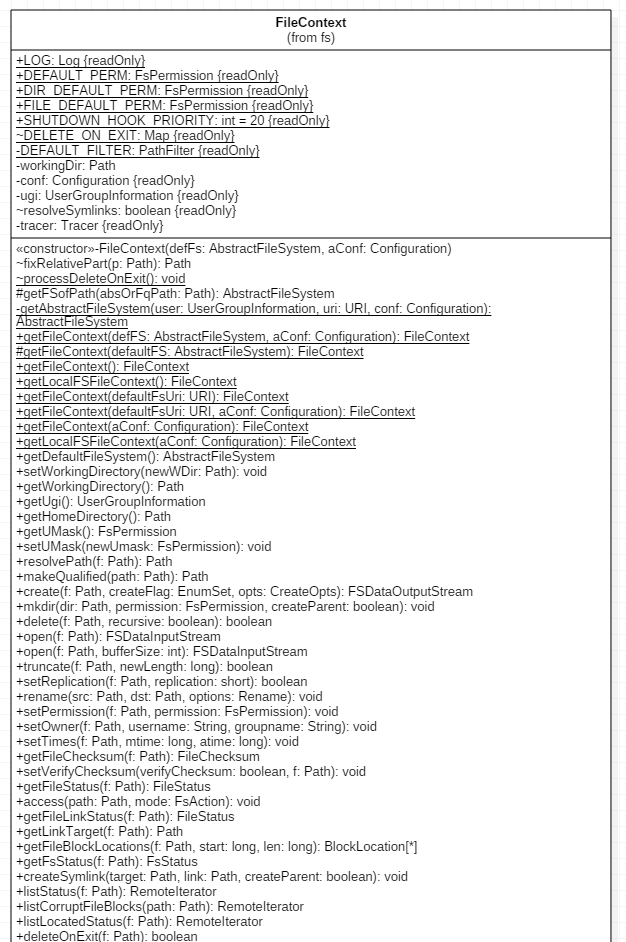
\includegraphics[width=1\linewidth]{UML/abstractfilesystem/FileContext1.PNG}
\caption{FileContext的UML类图1}
\label{fig:FileContext1}
\end{figure}

\begin{figure}
\centering
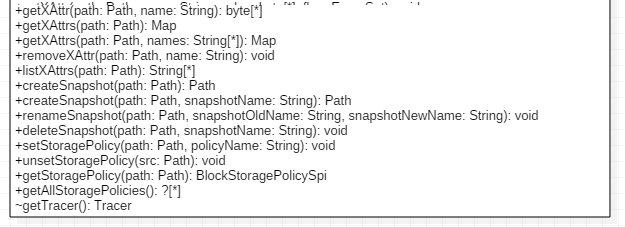
\includegraphics[width=1\linewidth]{UML/abstractfilesystem/FileContext2.PNG}
\caption{FileContext的UML类图2}
\label{fig:FileContext2}
\end{figure}

\subsubsection{getFileContext}
FileContext 由默认文件系统、工作目录和umask 定义。获得一个FileContext可以使用FileContext的静态方法:getFileContext();getLocalFSFileContext()
getFileContext有多重重载的形式。
\begin{quote}
示例1:使用从\verb|$HADOOP_CONFIG/core.xml|读取的默认配置。未指定的值来自发行版jar中的core-defaults.xml。
myFContext = FileContext.getFileContext();//使用默认配置//具有默认的FS
myFContext.create(path,…);
myFContext.setWorkingDir(路路径);
myFContext.open(path,…);…


示例2:获取具有特定URI的FileContext作为默认FS
myFContext = FileContext.getFileContext(URI);
myFContext.create(path,…);
\end{quote}

\subsubsection{Path Names}
Hadoop文件系统支持URI名称空间和URI名称。这使得要使用完全限定URI引用的多种类型的文件系统。
两个常见的Hadoop文件系统实现是
本地文件系统:file:/// path
HDFS文件系统:hdfs:// nnAddress:nnPort / path

Hadoop文件系统还支持URI之外的其他命名方案。
Hadoop具有默认文件系统的概念,这意味着默认URI方案和权限。这使得斜线相对名称有默认的FS,这对用户来说更为方便。
默认FS通常由用户环境设置,也可以手动指定。

Hadoop还支持工作目录相对的名称,它们是相对于当前工作目录(类似于Unix)的路径。工作目录可以在与默认FS不同的文件系统中。
因此,Hadoop路径名称可以指定为以下之一:
一个完全限定的URI:scheme:// authority / path(例如, hdfs:// nnAddress:nnPort / foo / bar)
斜线相对名称:相对于默认文件系统的路径(例如, / foo / bar)
工作目录相对名称:相对于工作目录的路径(例如, foo / bar)
scheme(scheme:foo / bar)的相对路径是非法的。

\subsubsection{FileContext的属性}
FileContext是Unix中每个进程文件相关状态的模拟。它包含两个属性:
默认文件系统(用于解析斜杠相对名称)
umask(用于文件权限)
一般来说,这些属性是在用户的环境中从默认配置文件获得的。
在服务器端指定了进一步的文件系统属性。文件系统操作默认使用这些服务器端默认值,除非另有说明指定。
文件系统相关的服务器端默认值为:
主目录(默认为“/ user / userName”)
初始wd(仅适用于本地fs)
复制因子
块大小
缓冲区大小
encryptDataTransfer
校验和选项。 (checksumType和bytesPerChecksum)

\subsubsection{open}
FileContext 中的很多方法是用来取代FileSystem中的方法的。包括create,mkdir,delete,open,setReplication,rename,setPermission,setOwner,setTimes,getFileStatus,getFileLinkStatus,getLinkTarget,getFileBlockLocations 等方法在AbstractFileSystem 中都有对应的方法。这些方法的实现具有相同的形式。比如open 方法的代码如下:
\begin{java}
/**
   * Opens an FSDataInputStream at the indicated Path using
   * default buffersize.
   */
 public FSDataInputStream open(final Path f) throws AccessControlException,
      FileNotFoundException, UnsupportedFileSystemException, IOException {
    final Path absF = fixRelativePart(f);
    return new FSLinkResolver<FSDataInputStream>() {
      @Override
      public FSDataInputStream next(final AbstractFileSystem fs, final Path p)
        throws IOException, UnresolvedLinkException {
        return fs.open(p);
      }
    }.resolve(this, absF);
  }

  /**
   * Opens an FSDataInputStream at the indicated Path.
   */
  public FSDataInputStream open(final Path f, final int bufferSize)
      throws AccessControlException, FileNotFoundException,
      UnsupportedFileSystemException, IOException {
    final Path absF = fixRelativePart(f);
    return new FSLinkResolver<FSDataInputStream>() {
      @Override
      public FSDataInputStream next(final AbstractFileSystem fs, final Path p)
        throws IOException, UnresolvedLinkException {
        return fs.open(p, bufferSize);
      }
    }.resolve(this, absF);
  }
\end{java}
FileContext.open是通过调用AbstractFileSystem.open来实现的。

open操作的时序图示例:
图 \ref{fig:sequence} 是这个类的层次结构图。
\begin{figure}
\centering
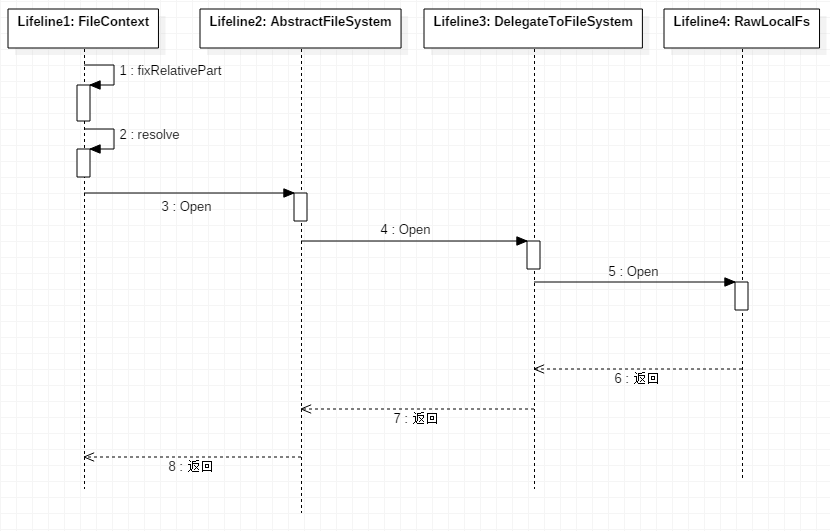
\includegraphics[width=1\linewidth]{UML/abstractfilesystem/sequence.PNG}
\caption{open操作的时序图}
\label{fig:sequence}
\end{figure}

